\documentclass[tikz,border=6pt]{standalone}
\usepackage{fontspec}
\setmainfont{Latin Modern Sans}
\usetikzlibrary{positioning,arrows.meta,fit,backgrounds}
\definecolor{tinte}{HTML}{222222}
\definecolor{blau}{HTML}{2A6FDB}
\definecolor{hell}{HTML}{EEF3FB}
\definecolor{rot}{HTML}{C0392B}
\definecolor{rothell}{HTML}{FBECEA}
\definecolor{grau}{HTML}{777777}
\begin{document}
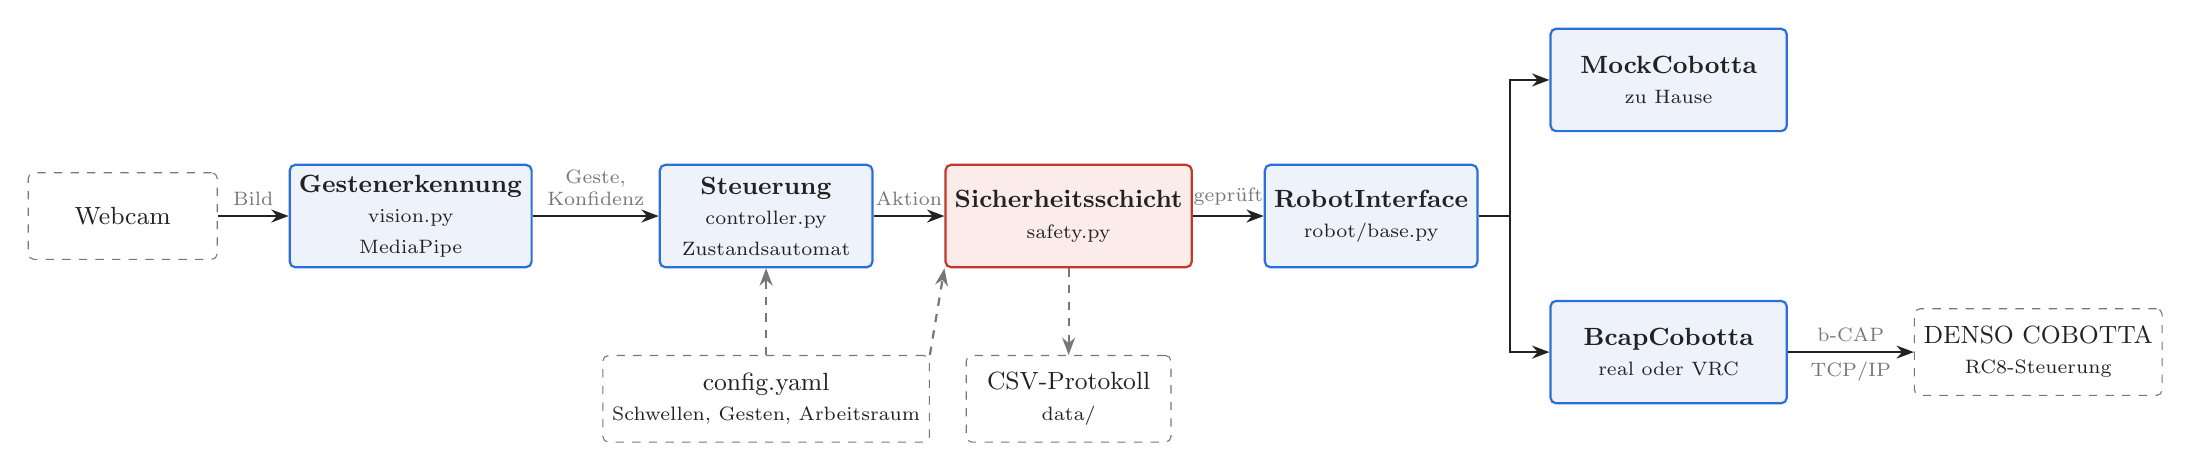
\begin{tikzpicture}[
  font=\small, node distance=7mm and 9mm,
  box/.style={draw=blau, fill=hell, rounded corners=2pt, align=center, minimum height=13mm, minimum width=27mm, text=tinte, line width=0.8pt},
  safe/.style={box, draw=rot, fill=rothell},
  ext/.style={draw=grau, rounded corners=2pt, align=center, minimum height=11mm, minimum width=24mm, text=tinte, dashed},
  pfeil/.style={-{Stealth[length=2.2mm]}, line width=0.8pt, draw=tinte},
  lbl/.style={font=\scriptsize, text=grau, align=center}
]
\node[ext] (cam) {Webcam};
\node[box, right=of cam] (vis) {\textbf{Gestenerkennung}\\ \scriptsize vision.py\\ \scriptsize MediaPipe};
\node[box, right=16mm of vis] (ctl) {\textbf{Steuerung}\\ \scriptsize controller.py\\ \scriptsize Zustandsautomat};
\node[safe, right=of ctl] (saf) {\textbf{Sicherheitsschicht}\\ \scriptsize safety.py};
\node[box, right=of saf] (rif) {\textbf{RobotInterface}\\ \scriptsize robot/base.py};
\node[box, above right=4mm and 9mm of rif, minimum width=30mm] (mock) {\textbf{MockCobotta}\\ \scriptsize zu Hause};
\node[box, below right=4mm and 9mm of rif, minimum width=30mm] (bcap) {\textbf{BcapCobotta}\\ \scriptsize real oder VRC};
\node[ext, right=16mm of bcap, minimum width=26mm] (rob) {DENSO COBOTTA\\ \scriptsize RC8-Steuerung};

\draw[pfeil] (cam) -- node[lbl, above]{Bild} (vis);
\draw[pfeil] (vis) -- node[lbl, above]{Geste,\\Konfidenz} (ctl);
\draw[pfeil] (ctl) -- node[lbl, above]{Aktion} (saf);
\draw[pfeil] (saf) -- node[lbl, above]{geprüft} (rif);
\draw[pfeil] (rif.east) -- ++(4mm,0) |- (mock.west);
\draw[pfeil] (rif.east) -- ++(4mm,0) |- (bcap.west);
\draw[pfeil] (bcap) -- node[lbl, above]{b-CAP}node[lbl, below]{TCP/IP} (rob);

\node[ext, below=11mm of ctl, minimum width=30mm] (cfg) {config.yaml\\ \scriptsize Schwellen, Gesten, Arbeitsraum};
\node[ext, below=11mm of saf, minimum width=26mm] (log) {CSV-Protokoll\\ \scriptsize data/};
\draw[pfeil, draw=grau, dashed] (cfg.north) -- (ctl.south);
\draw[pfeil, draw=grau, dashed] (cfg.north east) -- (saf.south west);
\draw[pfeil, draw=grau, dashed] (saf.south) -- (log.north);
\end{tikzpicture}
\end{document}
